\documentclass[2pt,a4paper]{article}
\usepackage[utf8]{inputenc}
\usepackage[french]{babel}
\usepackage[T1]{fontenc}
\usepackage{amsmath}
\usepackage{amsfonts}
\usepackage{amssymb}
\usepackage{graphicx}
\usepackage{epstopdf}
\usepackage{lmodern}
\usepackage{eurosym}
\usepackage{textcomp}
\usepackage{subfigure}
\usepackage{placeins}
\usepackage{listings}
\usepackage{proof}
\usepackage{amsthm}
\usepackage[left=1cm,right=1cm,top=2cm,bottom=1cm]{geometry}
\usepackage{color}
\usepackage{multicol}
\usepackage{fancyhdr}
\usepackage{tikz}

\tikzstyle{vertex}=[circle,fill=gray!50,minimum size=15pt,inner sep=0pt]
\tikzstyle{visited}=[circle,fill=green!25,minimum size=15pt,inner sep=0pt]
\tikzstyle{unvisited}=[circle,fill=blue!25,minimum size=15pt,inner sep=0pt]

\newcommand{\W}{\ {\color{red} \textbf{!!}} \ }

\setlength{\headsep}{0.2in}
\definecolor{listinggray}{gray}{0.9}
\definecolor{lbcolor}{rgb}{0.9,0.9,0.9}
\definecolor{mygreen}{rgb}{0,0.6,0}
\definecolor{mygray}{rgb}{0.5,0.5,0.5}
\definecolor{mymauve}{rgb}{0.58,0,0.82}

\pagestyle{fancy}
\fancyhf{}
\renewcommand{\sectionmark}[1]{\markright{#1}}
\fancyhead[RO]{\textbf{\thepage}}
\fancyhead[LO]{Université Catholique de Louvain}
%\fancyhead[RE]{\textsl{\leftmark}}
\renewcommand{\headrulewidth}{1px}

\lstset{ %
  backgroundcolor=\color{white},
  basicstyle=\footnotesize,
  breakatwhitespace=false,
  breaklines=true,
  captionpos=b,
  commentstyle=\color{mygreen},
  deletekeywords={},
  escapeinside={\%*}{*)},
  extendedchars=true,
  frame=none,
  keepspaces=true,
  keywordstyle=\color{blue},
  language=Java,
  morekeywords={},
  numbers=none,
  numbersep=0pt,
  numberstyle=\tiny\color{mygray},
  rulecolor=\color{black},
  showspaces=false,
  showstringspaces=false,
  showtabs=false,
  stepnumber=0,
  stringstyle=\color{mymauve},
  tabsize=2,
  belowskip=0pt,
  aboveskip=0pt,
}
\setlength{\parindent}{0cm}
\setlength{\columnseprule}{1px}
\author{François Aubry, Guillaume Derval, Benoît Legat, Anthony Gégo}
\title{Formulaire BAPC}
\begin{document}
\begin{multicols}{2}
{\Huge Formulaire BAPC 2013}\\
{\Large Team UCooL}\\
Auteurs: François Aubry, Guillaume Derval, Benoît Legat, Anthony Gégo.
\tableofcontents
\section{Remarks}
\subsection{Warning!}
\begin{enumerate}
	\item Read every statement!
	\item Do not copy-paste without thinking about it.
	\item Be careful of overflows! Use long! 
\end{enumerate}
 
\subsection{Operations on bits}
\begin{enumerate}
	\item Check parity of $n$: \lstinline{(n & 1) == 0}
	\item $2^n$: \lstinline|1 << n|.
	\item Test of the $i$th bit of $n$ is $0$: \lstinline{(n & 1 << i) != 0}
	\item Set the $i$th bit of $n$ at 0: \lstinline{n &= ~(1 << i)}
	\item Set the $i$th bit of $n$ at 1: \lstinline{n |= (1 << i)}
	\item Union: \lstinline{a | b}
	\item Intersection: \lstinline{a & b}
	\item Subtraction bits: \lstinline{a & ~b}
	\item Verify if $n$ is a power of 2: \lstinline{(n & (n-1) == 0)}
	\item Least significant bit not null of $n$: \lstinline{(n & (-n))}
	\item Negate: \lstinline{0x7fffffff^n}
\end{enumerate}

\subsection{Complexity table}
\begin{center}
\begin{tabular}{|c|c|}
\hline
n $\leq$ & Maximum complexity\\
\hline
$[10,11]$ & $O(n!),O(n^6)$ \\
$[15,18]$ & $O(2^n n^2)$\\
$[18,22]$ & $O(2^n n)$\\
$100$ & $O(n^4)$\\
$400$ & $O(n^3)$\\
$2K$ & $O(n^2\log(n))$\\
$10K$ & $O(n^2)$\\
$1M$ & $O(n\log(n))$\\
$10M$ & $O(n),O(\log(n)),O(1)$\\
\hline
\end{tabular}
\end{center}
\section{Graphes}
\subsection{Bases}
\begin{itemize}
\item Adjacency matrix: $A[i][j] = 1$ if $i$ is connected to $j$ and $0$ otherwise
\item Undirected graph: $A[i][j] = A[j][i]\ \forall\ i,j$ ($A = A^T$)
\item Adjacency list: \lstinline|LinkedList<Integer>[] g;|
$g[i]$ stores all neighbors of $i$
\item Useful alternatives: 
\begin{lstlisting}
HashSet<Integer>[] g; // for edge deletion
HashMap<Integer, Integer>[] g; // for weighted graph
\end{lstlisting}
\item Base classes
\begin{lstlisting}
class Vertex implements Comparable<Vertex> {
  int i; long d;
  public Vertex(int i, long d) { 
  	this.i = i; this.d = d;
  }
  public int compareTo(Vertex o) {
  	return d < o.d ? -1 : d > o.d ? 1 : 0;
  }
}

class Edge implements Comparable<Edge> {
  int o, d, w;
  public Edge(int o, int d, int w) {
    this.o = o; this.d = d; this.w = w;
  }
  public int compareTo(Edge o) {
    return w - o.w;
  }
}
\end{lstlisting}
\end{itemize}
\subsection{BFS}
Computes $d$, an array of distance from start vertex $v$.
$d[v]=0$, $d[u]=\infty$ if $u$ not connected to $v$. If $(u, w)\in E$ and $d[u]$ known and $d[w]$ unknown, $d[w] = d[u]+1$.\\

\lstinputlisting{Graphes/bfsvisit.java}
\subsubsection{Connected components}
\lstinputlisting{Graphes/bfs.java}
\subsubsection{Bipartite graph}
\lstinputlisting{Graphes/isBipartite.java}
\subsection{DFS}
Equals to BFS with \textit{Stack} instead of \textit{Queue} or recursive implementation. Complexity $O(|V|+|E|)$\\
\lstinputlisting{graphs/dfs.java}
\subsubsection{Topological order}
Graph must be acyclic. \\

\lstinputlisting{graphs/toposort.java}
\subsubsection{Strongly connected components}
Uses BFS following the topologic order. \\

\lstinputlisting{graphs/scc.java}
\subsubsection{SCC, Bridges and Articulation Points in C}
C version of SCC (shorter).

\lstinputlisting{graphs/scc1.cpp}

Bridges are edges that, when removed, increases the number of connected components. Articulation points are the same, but for vertices.

\lstinputlisting{graphs/scc2.cpp}

\subsubsection{Directed Graph to toposorted DAG}
In $O(n + m)$, with Tarjan SCC algo,
we merge the SCCs and take the resulting DAG,
(remembering their size in \lstinline|scc_size|)
which is reverse toposorted (i.e. node 0 has no outgoing edge),
ready for bottom up DP (starting with node 0 ending with node $N$) !

\lstinputlisting{graphs/sccdag.java}

\subsection{Minimum Spanning Tree}
\subsubsection{Prim}
\lstinputlisting{Graphs/prim.java}
\subsubsection{Kruskal}
Uses Union-Find (See section \ref{unionFind}).
\lstinputlisting{Graphs/kruskal.java}
\subsection{Dijkstra}
Shortest path from a node $v$ to other nodes. Graph must not have any negative weighted cycle.\\

\lstinputlisting{Graphs/dijkstra.java}
\subsection{Bellman-Ford\label{BellmanFord}}
Shortest path from a node $v$ to other nodes. Graph can have negative weighted cycles: Bellman-Ford won't give the correct shortest path, but will warn that a negative cycle exists. 
\lstinputlisting{Graphs/bellmanford.java}
\subsection{Floyd-Warshall}
Shortest path from a node $v$ to other nodes. Graph can have negative weighted cycles: Floyd-Warshall won't give the correct shortest path, but will warn that a negative cycle exists. Negative weighted cycles exists iif $result[v][v]<0$. $O(|V|^3)$ in time and $O(|V|^2)$ in memory.\\
\lstinputlisting{Graphs/floydwarshall.java}
\subsection{Max flow}
\subsubsection{Edmonds-Karps (BFS)}
Path in residual graph searched via BFS. $O(|V||E|^2)$.\\
\lstinputlisting{Graphs/edmondskarps.java}
\subsubsection{Ford-Fulkerson}
Equals to Edmonds-Karps, vut with a DFS. $O(|E|f^*)$ where $f^*$ is the value of the max flow.
\lstinputlisting{Graphs/maxflowslower.java}
\subsubsection{Min cut}
We search, between two nodes $s$ and $t$, $V_1$ and $V_2$ so as $s\in V_1$, $t\in V_2$ and $\sum_{e \in E(V_1, V_2)} w(e)$ minimum.\\
We just have to compute the max-flow between $s$ and $t$ and to apply a BFS/DFS on the residual graph. All node which are visited are in $V_1$, others in $V_2$. The weight from the cut is the max-flow.
\subsubsection{Maximum weighted bipartite matching}
(Assignment problem)
\lstinputlisting{Graphs/mwbm.java}
\section{Dynamic programming}
\subsection{Bottom-up}
Give n objects of value $v[i]$ to 3 people such that $\max_i V_i - \min_i V_i$ is minimum ($V_i$ is total value for person $i$).

$canDo[i][v_1][v_2]$ =  1 if we can give the objects $0, 1, \ldots, i$ such that $v_1$ is going to $P_1$ and $v_2$ to $P_2$, 0 otherwise. $v_3$ is determined from the sum.

\begin{minipage}{0.25\textwidth}
\textbf{Base case $i = 0$:}
\begin{itemize}
\item $ canDo[0][0][0]  = 1$
\item $ canDo[0][v[0]][0]  = 1$ 
\item $ canDo[0][0][v[0]]  = 1$
\end{itemize}
\end{minipage}
\begin{minipage}{0.25\textwidth}
\textbf{Case $i \geq 1$:} 

$ canDo[i][v_1][v_2] =  \\\text{\ \ }canDo[i - 1][v_1][v_2] \vee \\  \text{\ \ }canDo[i - 1][v_1 - v[i]][v_2] \vee \\  \text{\ \ } canDo[i - 1][v_1][v_2 - v[i]] $
\end{minipage}
\newline
\textbf{Sol. :} $ \min_{v_1, v_2 : canDo[n - 1][v_1][v_2]} \quad [max(v_1, v_2, S - v_1 - v_2) - min(v_1, v_2, S - v_1 - v_2)]$
\newline
\begin{lstlisting}
int solveDP() {
  boolean[][][] canDo = new boolean[v.length][sum + 1][sum + 1];
  // initialize base cases
  canDo[0][0][0] = true;
  canDo[0][v[0]][0] = true;
  canDo[0][0][v[0]] = true;
  // compute solutions using recurrence relation
  for(int i = 1; i < v.length; i++) {
    for(int a = 0; a <= sum; a++) {
      for(int b = 0; b <= sum; b++) {
        boolean giveA = a - v[i] >= 0 && canDo[i - 1][a - v[i]][b];
        boolean giveB = b - v[i] >= 0 && canDo[i - 1][a][b - v[i]];
        boolean giveC = canDo[i - 1][a][b];
        canDo[i][a][b] = giveA || giveB || giveC;
      }
    }
  }
  // compute best solution
  int best = Integer.MAX_VALUE;
  for(int a = 0; a <= sum; a++) {
    for(int b = 0; b <= sum; b++) {
      if(canDo[v.length - 1][a][b]) {
        best = Math.min(best, max(a, b, sum - a - b) - min(a, b, sum - a - b));
      }
    }
  }
  return best;
}
\end{lstlisting}
\subsection{Top-down}
Same problem as bottom-up. Main idea : memoization (Remember intermediate results).
\newline
\begin{lstlisting}
int solve(int i, int a, int b) {
  if(i == n) {
    memo[i][a][b] = max(a, b, sum - a - b) - min(a, b, sum - a - b);
    return memo[i][a][b]; 
  }
  if(memo[i][a][b] != null) {
    return memo[i][a][b];
  }
  int giveA = solve(i + 1, a + v[i], b);
  int giveB = solve(i + 1, a, b + v[i]);
  int giveC = solve(i + 1, a, b);
  memo[i][a][b] = min(giveA, giveB, giveC);
  return memo[i][a][b];
}
\end{lstlisting}
\subsection{Knapsack problem}
Given $n$ objects of value $v[i]$ and weight$w[i]$, an integer $W$ :
\begin{itemize}
\item Maximize  $\sum_i x[i] v[i]$
\item Such that $\sum_i x[i] w[i] \leq W$ \hspace{15pt} where $ x[i] $= 0 (not taken) or 1 (taken)
\end{itemize}
\subsubsection{No repetition}
best[i][w]= best way to take objects $0, 1, \ldots, i$ in a knapsack of capacity $w$.

\begin{minipage}{0.25\textwidth}
\textbf{Base case:}
\begin{itemize}
\item $best[0][w] = v[0]$ \\si $w[0] \leq w$
\item 0 else
\end{itemize}
\end{minipage}
\begin{minipage}{0.25\textwidth}
\textbf{Other cases:}\\
$best[i][w]   = \\ \text{\ \ }\max \{ best[i-1][w], \\ \text{\ \ \ \ }best[i-1][w-w[i]] + v[i] \}$
\end{minipage}
\subsubsection{An object can be repeated}
\begin{itemize}
\item $ best[0] = 0$
\item $best[w] = \max_{i : w[i] < w} \{best[w - w[i]] + v[i]\}$
\end{itemize}

\subsubsection{Several knapsacks}

$best[i][w_1][w_2] =$ best way to take objects $0, 1, \ldots, i$ in knapsacks of capacity $w_1$ and $w_2$.
\subsection{Longest common sub-sequence (LCS)}
Given two String $x$ and $y$. Find the longest common sub-sequence between $x$ and $y$.
 
\begin{center}
\begin{tikzpicture}[scale = 0.7]
\node at (-1, 1) {$x$};
\node at (-1, 0) {$y$};

\node[draw, circle] at (0, 0) (A)                  {\tiny G};
\node[draw, circle, fill = blue!25] at (1, 0) (B)  {\tiny C};
\node[draw, circle, fill = blue!25] at (2, 0) (C)  {\tiny A};
\node[draw, circle, fill = blue!25] at (3, 0) (D)  {\tiny A};
\node[draw, circle, fill = blue!25] at (4, 0) (E)  {\tiny G};
\node[draw, circle, fill = blue!25] at (5, 0) (F)  {\tiny T};
\node[draw, circle] at (6, 0) (G)                  {\tiny C};
\node[draw, circle, fill = blue!25] at (7, 0) (H)  {\tiny T};
\node[draw, circle, fill = blue!25] at (8, 0) (I)  {\tiny A};
\node[draw, circle, fill = blue!25] at (9, 0) (J)  {\tiny A};
\node[draw, circle, fill = blue!25] at (10, 0) (K) {\tiny T};
\node[draw, circle, fill = blue!25] at (11, 0) (L) {\tiny A};

\node[draw, circle, fill = blue!25] at (0, 1) (a)  {\tiny C};
\node[draw, circle, fill = blue!25] at (1, 1) (b)  {\tiny A};
\node[draw, circle, fill = blue!25] at (2, 1) (c)  {\tiny A};
\node[draw, circle] at (3, 1) (d)                  {\tiny G};
\node[draw, circle, fill = blue!25] at (4, 1) (e)  {\tiny G};
\node[draw, circle, fill = blue!25] at (5, 1) (f)  {\tiny T};
\node[draw, circle, fill = blue!25] at (6, 1) (g)  {\tiny T};
\node[draw, circle, fill = blue!25] at (7, 1) (h)  {\tiny A};
\node[draw, circle] at (8, 1) (i)  {\tiny T};
\node[draw, circle, fill = blue!25] at (9, 1) (j)  {\tiny A};
\node[draw, circle, fill = blue!25] at (10, 1) (k) {\tiny T};
\node[draw, circle, fill = blue!25] at (11, 1) (l) {\tiny A};

\draw (B) edge (a);
\draw (C) edge (b);
\draw (D) edge (c);
\draw (F) edge (f);
\draw (H) edge (g);
\draw (I) edge (h);
\draw (K) edge (k);
\draw (L) edge (l);
\draw (E) edge (e);
\draw (J) edge (j);

\end{tikzpicture}
\end{center}

\begin{itemize}
 \item \textbf{Formulation:}
$lcs[i][j] =$ size of \\\text{\ \ \ } $LCS(x[0] x[1] \cdots x[i - 1], y[0] y[1] \cdots y[j - 1])$
  \item \textbf{Base case:} $
lcs[0][j]  = 0$ \hspace{15pt} 
$lcs[i][0]  = 0$
  \item \textbf{Other cases: }
  \begin{itemize}
  \item Si $x[i-1] = y[i-1]$ alors: \\
  \quad $lcs[i][j] = 1 + lcs[i-1][j-1]$ 
  \item Si $x[i-1] \neq y[i-1]$ alors: \\
  \quad $lcs[i][j] = \max \{lcs[i-1][j], lcs[i][j-1]\}$
  \end{itemize}
\end{itemize}
\subsection{Matrix Chain Multiplication (MCM)}
Given a list of matrices, find the order minimizing the number of multiplications to compute their product.
\begin{itemize}
 \item Number to multiply a matrix of size $n \times m$ by a matrix of size $m \times r$ : $n \cdot m \cdot r$.

 \item Example: $A$ : $10 \times 30$, $B$ : $30 \times 5$ et $C$ : $5 \times 60$.
 \begin{itemize}
 \item For $(AB)C$ : $10 \cdot 30 \cdot 5 + 10 \cdot 5 \cdot 60 = 4500$ multiplications.
 \item For $A(BC)$ : $30 \cdot 5 \cdot 60 + 10 \cdot 30 \cdot 60 = 27000$ multiplications.
  \end{itemize}
\end{itemize}

\begin{itemize}
 \item \textbf{Formulation :}
 $best[i][j] =$ min cost to multiply $A_i, \ldots, A_j$
 \item \textbf{Base case :} $best[i][i] = 0 $
 \item \textbf{Other cases:}
 \begin{align*}
 best[i][j] = \min_{i \leq k < j} best[i][k] & + best[k + 1][j] \\
                                             & + A_i.n_1 \times A_k.n_2 \times A_j.n_2
 \end{align*}
\end{itemize}

\subsubsection{Generalized MCM}
Given a list of objects $x[0], \ldots, x[n - 1]$ and an operation $\odot$ with an associated cost, find the order in which perform the operations to minimize the total cost. The matrix product is replaced by $\odot$.

$$ best[i][j] = \min_{i \leq k < j} best[i][k] + best[k + 1][j] + cost(i, j, k)$$

$cost(i, j, k)$ is the cost of $(x[i] {\color{gray} \odot} \cdots {\color{gray} \odot} x[k]) {\color{blue} \mathbf{\odot}} (x[k + 1] {\color{gray} \odot} {\color{gray} \cdots} {\color{gray} \odot} x[j])$.
\newline
\begin{lstlisting}
int bestParenthesize() {
  int n = x.length; // x is a global variable
  int[][] best = new int[n][n];
  for(int i = 0; i < n; i++) { 
    best[i][i] = 0;
  }
  for(int l = 1; l <= n; l++) {
    for(int i = 0; i < n - l; i++) {
      int j = i + l;
      int min = Integer.MAX_VALUE;
      for(int k = i; k < j; k++) {
        min = Math.min(min, best[i][k] + best[k + 1][j] + cost(i, j, k)); // cost is problem-independent
      }
      best[i][j] = min;
    }
  }
  return best[0][n - 1];
} 
\end{lstlisting}
\subsection{Edit distance}
Given two String $x$ and $y$, by performing operations on en $x$, compute the minimal cost to transform $x$ into $y$.

We can (operation cost):
\begin{enumerate}
 \item Remove a character (D=1)
 \item Insert a character (I=1)
 \item Replace a character(R=2)
\end{enumerate}

\begin{itemize}
 \item \textbf{Formulation}:$
 editDist[i][j] $= min. cost to transform $x_0 \cdots x_{i - 1}$ into $y_0 \cdots y_{j - 1}$
 \item \textbf{Base case}: \\$ editDist[i][0] = i \cdot D \hspace{15pt}
 editDist[0][j] = j \cdot I$
 \item \textbf{Other cases}:
 \begin{align*}
 editDist[i][j] = \min  \quad  & editDist[i - 1][j] + D, \\
                               & editDist[i][j - 1] + I, \\
                               & editDist[i - 1][j - 1] + R^*
 \end{align*}
 where $R^* = R$ if $x[i-1] \neq y[j-1]$, $0$ else.
\end{itemize}
\ \newline
\begin{lstlisting}
int editDistance(String txt1, String txt2, int I, int D, int R){
  int[][] d = new int[txt1.length()+1][txt2.length()+1];
  for(int i=0; i <= txt1.length(); i++)
    d[i][0]=i*D;
  for(int j=0; j <= txt2.length(); j++)
    d[0][j]=j*I;
  for(int i=1; i <= txt1.length(); i++){
    for(int j=1; j <= txt2.length(); j++){
      int cost;
      // Non-equality cost
      if(txt1.charAt(i-1)==txt2.charAt(j-1))
        cost = 0;
      else
        cost = R;
      // Deletion, Insertion, Replacement
      d[i][j] = Math.min(Math.min(d[i-1][j] + D, d[i][j-1] + I), d[i-1][j-1] + cost);
    }
  }
  // Last computed element is the edit distance
  return d[txt1.length()][txt2.length()];
}
\end{lstlisting}
\subsection{Suffix array}

\includegraphics[width=\linewidth]{suffixarray.jpg}
\subsubsection{$O(n\log(n)^2)$, full matrix, need $n \leq 10K$}
\begin{itemize}
\item Suffix array of $algorithm$ = algorithm, gorithm, hm, ithm, lgorithm, m, orithm, rithm, thm

\item Characterized by its starting index\\
Example : Suffix array of $algorithm$: $$[0, \ 2, \ 7, \ 5, \ 1, \ 8, \ 3, \ 4, \ 6]$$
Example : Given $suf_j$ suffix beginning at index $j$, and $C(i, j, k)$ comparison result of $suf_j$ and $suf_k$ on the $2^i$ first characters.
\begin{align*}
C(i, j, k) = & \ C(i - 1, j, k) \hspace{15pt} \text{si $C(i - 1, j, k) \neq 0$} \\
             & \ C(i - 1, j + 2^{i - 1}, k + 2^{i - 1}) \hspace{15pt} \text{else}
\end{align*}

\end{itemize}
\begin{itemize}

\item Define a matrix $so$ such that:
\begin{align*}
so[i][j] = so[i][k] & \Leftrightarrow C(i, j, k) = 0 \\
so[i][j] < so[i][k] & \Leftrightarrow C(i, j, k) < 0 \\
so[i][j] > so[i][k] & \Leftrightarrow C(i, j, k) > 0 
\end{align*}

$so[i]$ is the order of sorted suffixes on the $2^i$ first characters.

\end{itemize}

\begin{itemize}

\item\textbf{Base case: }$so[0][j] = (int)s.charAt(i) $\\
Example: for $s = ccacab$ we have \\$ s[0] = [97, 97, 95, 97, 95, 96]$
\item For every $j$ we define a triplet $(l, r, j)$:
\begin{align*}
(s[i - 1][j], s[i - 1][j + 2^{i - 1}], j) & \quad \text{si $j + 2^{i - 1} < n$} \\
(s[i - 1][j], -1, j) & \quad \text{si $j + 2^{i - 1} \geq n$}
\end{align*}

\end{itemize}
\ \newline
\begin{lstlisting}
class Triple implements Comparable<Triple> {
  int l, r, index;
  public Triple(int half1, int half2, int index) {
    this.l = half1;
    this.r = half2;
    this.index = index;
  };
  public int compareTo(Triple other) {
    if(l != other.l) {
      return l - other.l;
    }
    return r - other.r;
  }
} 
\end{lstlisting}
\ \newline
\begin{lstlisting}
int[][] suffixOrder(String s) { // O(n log^2(n))
  int n = s.length();
  int lg = (int)Math.ceil((Math.log(n) / Math.log(2))) + 1;
  int[][] so = new int[lg][n];
  // initialize so[0] with character order
  for(int i = 0; i < n; i++) {
    so[0][i] = s.charAt(i);
  }
  Triple[] next = new Triple[n];
  for(int i = 1; i < lg; i++) {
    // build the next array
    for(int j = 0; j < n; j++) {
      int k = j + (1 << (i - 1));
      next[j] = new Triple(so[i - 1][j], k < n ? so[i - 1][k] : -1, j);
    }
    // sort next array
    Arrays.sort(next);
    // build so[i]
    for(int j = 0; j < n; j++) {
      if(j == 0) {
      // smallest elements gets value 0 
      so[i][next[j].index] = 0;
     } else if(next[j].compareTo(next[j - 1]) == 0) {
      // equal to previous so it gets the same value
      so[i][next[j].index] = so[i][next[j - 1].index];
     } else {
      // largest than previous so get + 1
      so[i][next[j].index] = so[i][next[j - 1].index] + 1;
     }
   }
 }
 return so;
}

//Calcule le Suffix Array pour un so donne:
int[] suffixArray(int[][] so) {
  int[] sa = new int[so[0].length];
  for(int j = 0; j < so[0].length; j++) {
    sa[so[so.length - 1][j]] = j;
  }
  return sa;
}

//Retourne le plus long prefixe commun de suf_j (le suffixe de s commencant a j = s.substr(j)) et suf_k pour un so donne:
int lcp(int[][] so, int j, int k) { // O(log(n)
  int lcp = 0;
  int n = so[0].length;
  for(int i = so.length - 1; i >= 0; i--) {
    if(j < n && k < n && so[i][j] == so[i][k]) {
      lcp += (1 << i);
      j += (1 << i);
      k += (1 << i);
    }
  }
  return lcp;
}

//Quelques exemples
String maxStrRepeatedKTimes(String s, int k) {
  int[][] so = suffixOrder(s);
  int[] SA = suffixArray(so);
  int n = s.length();
  int max = Integer.MIN_VALUE;
  int j = 0;
  for(int i = 0; i <= n - k; i++) {
    int lcp = lcp(so, SA[i], SA[i + k - 1]);
    if(lcp > max) {
      max = lcp;
      j = SA[i];
    }
  }
  return s.substring(j, j + max);
}
	
String minLexicographicRotation(String s) {
  int n = s.length();
  s += s;
  int[] SA = suffixArray(suffixOrder(s));
  int i = 0;
  while(!(0 <= SA[i] && SA[i] < n)) {
    i++;
  }
  return s.substring(SA[i], SA[i] + n);
}

class MaxLexConc implements Comparator<String> {
 public int compare(String x, String y) {
    String xy = x + y;
    String yx = y + x;
    if(xy.compareTo(yx) < 0 || 
      (xy.equals(yx) && x.length()<y.length())) {
      return 1; 
    }
    return -1; 
}
\end{lstlisting}

\subsubsection{$O(n\log(n))$, only last line, need $n \leq 100K$}
\lstinputlisting{DP/suffixArray.java}


\section{Geometry}
Be careful of rounding errors. Define $E$ in function of the problem.
\lstinline|Double.parseDouble| est bien plus lent que \lstinline|Integer.parseInt|.
\begin{lstlisting}
boolean eq(double a,double b){return Math.abs(a - b) <= E;}
boolean le(double a,double b){return a < b - E;}
boolean leq(double a,double b){return a <= b + E;}
\end{lstlisting}
\subsection{Vectors}
\subsubsection{Rotation around (0,0)}
$(x, y) \leftrightarrow x + y i$\\
$\rho e^{i\theta} = \rho \cos(\theta) + i \rho \sin(\theta)$\\

$(x, y)$ rotated by $\alpha$ is
$(\cos(\alpha) x - \sin(\alpha) y, \sin(\alpha)  x + \cos(\alpha) y)$
\subsection{Points}
\begin{lstlisting}
class Point implements Comparable<Point>
{
  double x, y;
  public int compareTo(Point o) { //xcomp
    if(a.x < b.x) return -1;
    if(a.x > b.x) return 1;
    if(a.y < b.y) return -1;
    if(a.y > b.y) return 1;
    return 0;
  }
}

class yComp implements Comparator<Point> {
  public int compare(Point p, Point q) {
    if(p.y == q.y) {return Double.compare(p.x, q.x);}
    return Double.compare(p.y, q.y);
  }
}
\end{lstlisting}
\subsubsection{Point in box}
\begin{lstlisting}
boolean inBox(Point p1, Point p2, Point p) {
  return Math.min(p1.x, p2.x) <= p.x && p.x <= Math.max(p1.x, p2.x) &&			           
         Math.min(p1.y, p2.y) <= p.y && p.y <= Math.max(p1.y, p2.y);
}
\end{lstlisting}
\subsubsection{Polar sort}
\begin{lstlisting}
LinkedList<Point> sortPolar(Point[] P, Point o)
{
  LinkedList<Point> above = new LinkedList<Point>();
  LinkedList<Point> samePos = new LinkedList<Point>();
  LinkedList<Point> sameNeg = new LinkedList<Point>();
  LinkedList<Point> bellow = new LinkedList<Point>();
  for(Point p : P)
  {
    if(p.y > o.y)
      above.add(p);
    else if(p.y < o.y)
      bellow.add(p);
    else
    {
      if(p.x < o.x)
        sameNeg.add(p);
      else
        samePos.add(p);

    }
  }
  PolarComp comp = new PolarComp(o);    
  Collections.sort(samePos, comp);
  Collections.sort(sameNeg, comp);
  Collections.sort(above, comp);
  Collections.sort(bellow, comp);
  LinkedList<Point> sorted = new LinkedList<Point>();
  for(Point p : samePos) sorted.add(p);
  for(Point p : above) sorted.add(p);
  for(Point p : sameNeg) sorted.add(p);
  for(Point p : bellow) sorted.add(p);
  return sorted;
}

class PolarCmp implements Comparator<Point> {
  static Point orig = new Point(0, 0);
  public int compare(Point p, Point q) {
    double o = orient(orig, p, q);
    if(o == 0) {
      if(p.x * p.x + p.y * p.y > q.x * q.x + q.y * q.y)
        return 1;
      return -1;
    }
    return -(int)Math.signum(o);
  }
}
\end{lstlisting}
\subsubsection{Closest pair of points}
\begin{lstlisting}
double closestPair(Point[] points) {
  if(points.length == 1) {return Double.POSITIVE_INFINITY;}
  Arrays.sort(points, new xComp());
  double min = dist(points[0], points[1]);
  // keep track of the leftmost point
  int leftmost = 0;
  TreeSet<Point> candidates = new TreeSet<Point>(new yComp());
  candidates.add(points[0]);
  candidates.add(points[1]);
  for(int i = 2; i < points.length; i++) {
    Point cur = points[i];
    // eliminate points s.t cur.x - x > min 
    while(cur.x - points[leftmost].x > min) {
      candidates.remove(points[leftmost]);
      leftmost++;
    }
    Point low = new Point(0, cur.y - min);
    Point high = new Point(0, cur.y + min);
    // check all points in the rectangle
    for(Point point : candidates.subSet(low, high))
      min = Math.min(min, dist(cur, point));
    candidates.add(cur);
  }
  return min;
}
\end{lstlisting}
\subsubsection{Orientation}
$$
orient(p, q, r) = 
\begin{vmatrix}
1 & p_x & p_y \\
1 & q_x & q_y \\
1 & r_x & r_y
\end{vmatrix}
$$

$$
orient(p, q, r) \left\{
\begin{array}{l l l}
= 0 \quad & \text{$p, q, r$ are collinear} \\
< 0 \quad & \text{$p$ -> $q$ -> $r$ is clockwise} \\
> 0 \quad & \text{$p$ -> $q$ -> $r$ is counterclockwise}
\end{array} \right.
$$

$$
|orient(p, q, r)| = 2 \cdot area \ \triangle(p, q, r)
$$

\begin{lstlisting}
double orient(Point p, Point q, Point r) {
  return q.x * r.y - r.x * q.y - p.x * (r.y - q.y) + p.y * (r.x - q.x);
}
\end{lstlisting}
\subsubsection{Angle visibility}
$x$ lies strictly inside the angle formed by $p, q, r$ iff
\begin{align*}
sgn(orient(p, q, x)) & = sgn(orient(p, x, r)) \\
sgn(orient(p, r, x)) & = sgn(orient(p, x, q)) \\
\end{align*}
To allow it to lie on the border simply check if $$sgn(orient(p, q, x)) = 0 \text{ or } sgn(orient(p, r, x)) = 0$$
\subsubsection{Fixed radius neighbors (1D)}
\begin{lstlisting}
List<Double[]> findPairs1D(double[] x, double r) {
  HashMap<Integer, List<Double>> H = new HashMap<Integer, List<Double>>();
  // fill buckets
  for(int i = 0; i < x.length; i++) {
    int b = (int)(x[i] / r);
    if(H.containsKey(b)) {
      H.get(b).add(x[i]);
    } else {
      List<Double> L = new ArrayList<Double>();
      L.add(x[i]);
      H.put(b, L);				
    }
  }
  // find pairs in consecutive buckets
  List<Double[]> pairs = new LinkedList<Double[]>(); 
  for(int i = 0; i < x.length; i++) {
    int b = (int)(x[i] / r);
    List<Double> bucket = H.get(b + 1);
    if(bucket != null)
      for(double y : bucket)
        if(y - x[i] <= r)
          pairs.add(new Double[] {x[i], y});
  }
  // add points in buckets
  for(List<Double> bucket : H.values())
    for(int i = 0; i < bucket.size(); i++)
      for(int j = i + 1; j < bucket.size(); j++)
        pairs.add(new Double[] {bucket.get(i), bucket.get(j)});
  return pairs;
}
\end{lstlisting}
\subsubsection{Fixed radius neighbors (2D)}
\begin{lstlisting}
List<Point[]> findPairs2D(Point[] points, double r) {
  HashMap<Integer, List<Point>> H = new HashMap<Integer, List<Point>>();
  // fill buckets
  for(int i = 0; i < points.length; i++) {
    int bx = (int)(points[i].x / r);
    int by = (int)(points[i].y / r);
    int key = 33 * bx + by;
    if(H.containsKey(key)) {
      H.get(key).add(points[i]);
    } else {
      List<Point> L = new ArrayList<Point>();
      L.add(points[i]);
      H.put(key, L);				
    }
  }
  // find pairs in adjacent buckets
  List<Point[]> pairs = new LinkedList<Point[]>();
  int[][] dir = new int[][] {new int[] {1,0}, new int[] {0,1}, new int[] {1,1}};
  for(int i = 0; i < points.length; i++) {
    int bx = (int)(points[i].x / r);
    int by = (int)(points[i].y / r);
    for(int[] d : dir) {
      List<Point> bucket = H.get(33 * (bx + d[0]) + (by + d[1]));
      if(bucket != null)
        for(Point y : bucket)
          if(sqDist(points[i], y) <= r * r)
            pairs.add(new Point[] {points[i], y});					
    }
  }
  // add points in buckets
  for(List<Point> bucket : H.values())
    for(int i = 0; i < bucket.size(); i++)
      for(int j = i + 1; j < bucket.size(); j++)
        if(sqDist(bucket.get(i), bucket.get(j)) <= r * r)			
          pairs.add(new Point[] {bucket.get(i), bucket.get(j)});
  return pairs;
}
\end{lstlisting}

\subsection{Lines}
General equation:$Ax + By = C$. The line through $(x_1, y_1), (x_2, y_2)$ is given by: $A = y_2 - y_1$, $B = x_1 - x_2$, $C = A x_1 + B y_1$.
\subsubsection{Intersections}
Intersection exists there is a solution for $A_1 x + B_1 y = C_1$ and $A_2 x + B_2 y = C_2$. This happens if and only if $$d := \det \begin{pmatrix}
A_1 & B_1 \\
A_2 & B_2 \\
\end{pmatrix} \neq 0$$
Intersection is given by
$$\begin{pmatrix}
x\\
y
\end{pmatrix} = 
\begin{pmatrix}
A_1 & B_1 \\
A_2 & B_2 \\
\end{pmatrix}^{-1} 
\begin{pmatrix}
C_1 \\
C_2
\end{pmatrix}
=
\frac{1}{d}
\begin{pmatrix}
B_2 & -B_1 \\
-A_2 & A_1 \\
\end{pmatrix} 
\begin{pmatrix}
C_1 \\
C_2
\end{pmatrix}
$$
\subsubsection{Perpendicular line}
The lines perpendicular to $Ax + By = C$ are
$$-Bx + Ay = D \quad \text{for $D \in \mathbb{R}$}$$
If we want the one that goes through $(x_0, y_0)$ set
$$D = - B x_0 + A y_0$$
\subsubsection{Orthogonal Symmetry}
For a line, find $X'$, the point which is the orthogonal symmetry of $X$ on line $a$. \\
Computes the perpendicular of the given line that goes through $X$. Compute intersection $Y$. $X' = Y - (X - Y)$.
\subsection{Segments}
\subsubsection{Intersection}
\begin{itemize}
\item Treat segments as lines.
\item If $d \neq 0$, compute line intersection $(x, y)$.
\item Segments intersect iff
\begin{align*}
\min(x_1, x_2) \leq & \ x \leq \max(x_1, x_2) \\
\min(y_1, y_2) \leq & \ y \leq \max(y_1, y_2)
\end{align*}
\end{itemize}
\begin{lstlisting}
boolean intersects(Point p1, Point p2, Point p3, Point p4) {
  double o1 = orient(p1, p2, p3);
  double o2 = orient(p1, p2, p4);
  double o3 = orient(p3, p4, p1);
  double o4 = orient(p3, p4, p2);
  // check first condition of the lemma
  if(o1 * o2 < 0 && o3 * o4 < 0) return true;
  // check seconds condition of the lemma
  if(o1 == 0 && inBox(p1, p2, p3)) return true;
  if(o2 == 0 && inBox(p1, p2, p4)) return true;
  if(o3 == 0 && inBox(p3, p4, p1)) return true;
  if(o4 == 0 && inBox(p3, p4, p2)) return true;
  return false;
}
\end{lstlisting}
\subsubsection{Intersections problem}
Given a lot of segments, return true if it exists a pair that intersects.
\begin{lstlisting}
boolean segmentIntersection(Segment[] S) {
  Event[] events = new Event[2 * S.length];
  // create event points
  for(int i = 0, j = 0; i < S.length; i++) {
    events[j++] = new Event(S[i].l.x, true, S[i]);
    events[j++] = new Event(S[i].r.x, false, S[i]);
  }
  Arrays.sort(events);
  SegmentCmp cmp = new SegmentCmp();
  TreeSet<Segment> T = new TreeSet<Segment>(cmp);
  // sweep line
  for(Event event : events) {
    Segment s = event.s;
    cmp.x = event.x;
    if(event.isLeft) {
      // new segment found. check if it intersects one of its neighbors
      T.add(s);
      Segment above = T.higher(s);
      Segment bellow = T.lower(s);
      if((above != null && intersects(above, s)) || 
         (bellow != null && intersects(bellow, s)))
        return true;
    } else {
      // end of segment. check if its neighbors intersect
      Segment above = T.higher(s);
      Segment bellow = T.lower(s);
      if(above != null && bellow != null && intersects(above, bellow))
        return true;
      T.remove(s);
    }
  }
  return false;
}

class Event implements Comparable<Event> {
  double x;
  boolean isLeft;
  Segment s;
  public Event(double x, boolean isLeft, Segment s) {
    this.x = x;
    this.isLeft = isLeft;
    this.s = s;
  }
  public int compareTo(Event other) {
    int cmp = Double.compare(x, other.x);
    // ensure that left comes before right
    if(cmp == 0) return isLeft? -1 : 1;
    return cmp;
  }
  public String toString() {
    return x + " " + isLeft;
  }
}

class SegmentCmp implements Comparator<Segment> {
  double x;
  public int compare(Segment s1, Segment s2) {
    // compute A,B,C from eq Ax + by = C for each segment
    double A1 = s1.r.y - s1.l.y;
    double B1 = s1.l.x - s1.r.x;
    double C1 = A1 * s1.l.x + B1 * s1.l.y;

    double A2 = s2.r.y - s2.l.y;
    double B2 = s2.l.x - s2.r.x;
    double C2 = A2 * s2.l.x + B2 * s2.l.y;

    // no divisions =)
    double t1 = B2 * (C1 - A1 * x);
    double t2 = B1 * (C2 - A2 * x);
    if(t1 == t2) {
      return s1 == s2? 0 : -1;
    } else if(B1 * B2 > 0) {
      return Double.compare(t1, t2);
    } else {
      return Double.compare(t2, t1);
    }
  }
}
\end{lstlisting}
\subsection{Circles}
\subsubsection{Circles from 3 points}
\begin{itemize}
\item $3$ non collinear points define a unique circle.
\item $c = $ intersection of bisectors of $XY$ and $YZ$. 
\end{itemize}
\subsection{Polygon}
\subsubsection{Triangles}
\begin{itemize}
  \item côtés $a,b,c$, angles $A,B,C$, hauteurs $h_A,h_B,h_C$, $s=\frac{a+b+c}{2}$, aire $S$.
  \item Aire: $S=ah_A/2$, $S=ab\sin C/2$, $S=\sqrt{s(s-a)(s-b)(s-c)}$.
  \item Inradius $r=\frac{S}{s}$.
  \item Outradius $2R = \frac{a}{\sin A} = \frac{b}{\sin B} = \frac{c}{\sin C}$.
  \item $rR = \frac{abc}{4s}$.
\end{itemize}
\subsubsection{Check convexity}
\begin{lstlisting}
boolean isConvex(Point[] P) {
  if(P.length < 3) return false;
  double o1 = orient(P[P.length-1], P[0], P[1]);
  for (int i = 0; i < P.length; i++) {
    double o2 = orient(P[i], P[i + 1], P[i + 2]);
    if(o1 * o2  < 0) {
      return false;
    } else if (o2 != 0) {
      o1 = o2;
    }
  }
  return true;
}
\end{lstlisting}
\subsubsection{Winding number}
\begin{lstlisting}
// assumes p is not on P
double winding(Point[] P, Point p) {
  //make a translation so p = (0, 0)
  for(Point q : P) {
    q.x -= p.x;
    q.y -= p.y;
  }
  double w = 0;
  for(int i = 0; i < P.length - 1; i++) {
    if(P[i].y * P[i + 1].y < 0) {
      // segment crosses the x-axis
      double r = (P[i].y - P[i+1].y) * P[i].x + P[i].y * (P[i+1].x - P[i].x);
      //check for intersection with the positive x-axis
      if((P[i].y - P[i+1].y > 0 && r > 0) || (P[i].y - P[i+1].y < 0 && r < 0)) {
        // segment fully crosses the x-axis
        // - to + add 1, + to - subtract 1
        w += P[i].y < 0? 1 : -1;
      } else if(P[i].y == 0 && P[i].x > 0) {
        // the segment starts at the x-axis
        // 0 to + add 0.5, 0 to - subtract 0.5
        w += P[i+1].y > 0? 0.5 : -0.5;
      } else if(P[i+1].y == 0 && P[i+1].x > 0) {
        // the segment ends at the x-axis
        // - to 0 add 0.5, + to 0 subtract 0.5
        w += P[i].y < 0? 0.5 : -0.5;
      }
    }
  }
  return w;
}
\end{lstlisting}
\subsubsection{Convex Hull}
\begin{lstlisting}
Point[] convexHull(Point[] points) {
  // sort points by increasing x coordinates
  Arrays.sort(points, new xComp());
  // build upper chain
  Point[] upChain = buildChain(points, 1);
  // build lower chain
  Point[] loChain = buildChain(points, -1);
  Point[] hull = new Point[upChain.length + loChain.length - 2];
  int i;
  // build convex hull from upper and lower chain
  for(i = 0; i < upChain.length; i++) {
    hull[i] = upChain[i];
  }
  for(int j = loChain.length - 2; j >= 1; j--) {
    hull[i] = loChain[j];
  }
  return hull;
}

Point[] buildChain(Point[] points, int sgn) {
  Point[] S = new Point[points.length];
  int k = 0;
  S[k++] = points[0]; // push points[0]
  S[k++] = points[1]; // push points[1]
  // build chain
  for(int i = 2; i < points.length; i++) {
    //double orient = orient(S[k - 2], S[k - 1], points[i]);
    while(k >= 2 && sgn * orient(S[k - 2], S[k - 1], points[i]) >= 0) {
      S[k - 1] = null; // pop
      k--;
    }
    S[k++] = points[i]; // push points[i]
  }
  return Arrays.copyOf(S, k);
}
\end{lstlisting}

\subsection{Interval Tree}

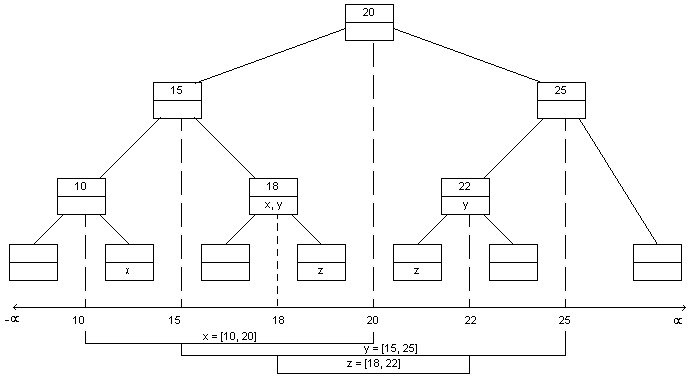
\includegraphics[scale=0.38]{Geometrie/it.png}

\lstinputlisting{Geometrie/intervaltree.java}

\subsection{Area of union of rectangles}

\lstinputlisting{Geometrie/rectangles.java}

\subsection{C library by Xiao}

\lstset{language=C}
{\setmainfont{CODE2000.TTF} % font that supports chinese
\lstinputlisting{Geometrie/Geometry.h}
}
\lstset{language=Java}

\section{Math}
\subsection{Permutations, Combinations, Arrangements... {\footnotesize \textit{untested}}}
\begin{lstlisting}
void nextPerm(int[] p) {
  int n = p.length;
  int k = n - 2;
  while(k >= 0 && p[k] >= p[k + 1]) {k--;}
  int l = n - 1;
  while(p[k] >= p[l]) {l--;}
  swap(p, k, l);
  reverse(p, k + 1, n);
}

LinkedList<Integer> getIPermutation(int n, int index) {
  LeftRightArray lr = new LeftRightArray(n);
  lr.freeAll();
  LinkedList<Integer> perm = new
  LinkedList<Integer>();
  getPermutation(lr, index, fact(n), perm);
  return perm;
}

void getPermutation(LeftRightArray lr, int i, long fact, LinkedList<Integer> perm) {
  int n = lr.size();
  if(n == 1) {
    perm.add(lr.freeIndex(0, false));
  } else {
    fact /= n;
    int j = (int)(i / fact);
    perm.add(lr.freeIndex(j, true));
    i -= j * fact;
    getPermutation(lr, i, fact, perm);
  }
}

int[] getICombinadic(int n, int k, long i) {
  int[] comb = new int[k];
  int j = 0;
  for(int z = 1; z <= n; z++) {
    if ( k == 0 ) {
      break;
    }
    long threshold = C(n - z, k - 1);
    if (i < threshold) {
      comb[j] = z - 1;
      j++;
      k = k - 1;
    } else if (i >= threshold) {
      i = i - threshold;
    }
  }
  return comb;
}

void combinations(int n, int k) {
  combinations(n, 0, new int[k], 0);
}

void combinations(int n, int j, int[] comb, int k) {
  if(k == comb.length) {
    System.out.println(Arrays.toString(comb));
  } else {
    for(int i = j; i < n; i++) {
      comb[k] = i;
      combinations(n, i + 1, comb, k + 1);
    }
  }
}
void subsets(int[] set) {
  int n = (1 << set.length);
  for(int i = 0; i < n; i++) {
    int[] sub = new int[Integer.bitCount(i)];
    int k = 0, j = 0;
    while((1 << j) <= i) {
      if((i & (1 << j)) == (1 << j)) {
        sub[k++] = set[j];
      }
      j++;
    }
    System.out.println(Arrays.toString(sub));
  }
}
\end{lstlisting}
\subsection{Decomposition in unit fractions {\footnotesize \textit{untested}}}
Write $0<\frac{p}{q}<1$ as a sum of $\frac{1}{k}$
\begin{lstlisting}
void expandUnitFrac(long p, long q) {
	if(p != 0) {
		long i = q % p == 0 ? q/p : q/p + 1;
		System.out.println("1/" + i);
		expandUnitFrac(p*i-q, q*i);
	}
}
\end{lstlisting}
\subsection{Combination}
Number of combinations of $k$ elements within $n$ ones ($C^k_n$)

Special case : $C^k_n\ mod\ 2 = n\oplus m$
\begin{lstlisting}
long C(int n, int k) {
  double r = 1;
  k = Math.min(k, n - k);
  for(int i = 1; i <= k; i++)
  r /= i;
  for(int i = n; i >= n - k + 1; i--)
  r *= i;
  return Math.round(r);
}
\end{lstlisting}
\subsubsection{Catalan numbers}
$\cat(n) = \frac{C_n^{2n}}{n+1}$ $\cat(n+1) = \frac{(2n+2)(2n+1)}{(n+2)(n+1)}\cat(n)$
\begin{itemize}
  \item distinct binary trees with $n$ vertices.
  \item expressions containing $n$ pairs of parentheses correctly matched (e.g. $n=3$ $()()(),()(()),(())(),((())),(()())$).
  \item parenthesize $n+1$ factors (e.g. $n=3$ $(ab)(cd),a(b(cd)),((ab)c)(d),(a(bc))(d),a((bc)d)$).
  \item triangulate a convex polygon of $n+2$ sides.
  \item number of monotonic paths along the edge of a $n\times n$ grid which do not pass above de diagonal.
\end{itemize}

\vspace{0.5cm}

Compute all Catalan number $\leq n$
\begin{lstlisting}
long[] allCatalan(int n) {
  long[] catalanNumbers = new long[n];
  catalanNumbers[0] = 1;
  for(int i = 1; i < n; i++) {
    int j = i - 1;
    long b = j * j;
    long a = 4 * b + 6 * j + 2;
    b += 3 * j + 2;
    catalanNumbers[i] = catalanNumbers[j] * a/b;
  }
  return catalanNumbers;
}
\end{lstlisting}


\subsection{Fibonacci series}
$f(0) = 0$, $f(1) = 1$ et $f(n) = f(n - 1) + f(n - 2)$.\\
The following relation enables us to compute every number of the series in $O(log(n))$ :\\
$$\begin{pmatrix}
1 & 1\\
1 & 0
\end{pmatrix}^n=\begin{pmatrix}
f_{n+1} & f_n\\
f_n & f_{n-1}
\end{pmatrix}$$
\subsection{Cycle finding}
\begin{lstlisting}
int[] floydCycleFinding (int x0) {
  int tortoise = f(x0), hare = f(f(x0));
  while (tortoise != hare) {
    tortoise = f(tortoise);
    hare = f(f(hare)); }
  int mu = 0; hare = x0; // first
  while (tortoise != hare) {
    tortoise = f(tortoise); hare = f(hare); mu++; }
  int lambda = 1; hare = f(tortoise); // length
  while (tortoise != hare) {
    hare = f(hare); lambda++; }
  return new int[] {mu, lambda};
}
\end{lstlisting}
\subsection{Number theory}
\subsubsection{Misc}
\[
  ax \leq b \Leftrightarrow x \leq \left\lfloor \frac{b}{a} \right\rfloor \quad
  ax \geq b \Leftrightarrow x \leq \left\lceil \frac{b}{a} \right\rceil \quad
  \left\lceil \frac{a}{b} \right\rceil = \left\lfloor \frac{a+b-1}{b} \right\rfloor.
\]
\begin{lstlisting}
long gcd (long a, long b) {
  return (b == 0) ? a : gcd(b, a % b);
}
long lcm (long a, long b) {
  return a * (b / gcd(a,b));
}
long modInverse (long a, long b) {
  return big(a).modInverse(big(b)).longValue();
}
long modInverse (long a, long b) {
  extendedEuclid(a, b);
  return x;
}
\end{lstlisting}
In prime factorization of $n$, the power of $p$ is
\[\sum_{i=1}^{\infty} \left\lfloor \frac{n}{p^i} \right\rfloor\]
\begin{lstlisting}
int factopower (int n, int p) {
  int pow = 0;
  while (n > 0) {
    pow += n / p;
    n /= p;
  }
  return pow;
}
\end{lstlisting}

\subsubsection{Équations diophantiennes}
$ax + by = c$. $d = \gcd(a,b)$, no sol si $d$ divise pas $c$ sinon $(a,b) = (x (n/d) + (b/d)n, y (n/d) + (a/d)n)$ où $ax + by = d$ $n \in \mathbb{Z}$.
\begin{lstlisting}
static int x, y;
static int extendedEuclid(int a, int b) {
  if (b == 0) { x = 1; y = 0; return a; }
  int d = extendedEuclid(b, a % b);
  int x1 = y;
  int y1 = x - (a / b) * y;
  x = x1;
  y = y1;
  return d;
}
\end{lstlisting}
\subsubsection{Chinese remainder theorem}
\begin{lstlisting}
static long[] chinese (long[] b, long[] m) {
  long x = b[0], l = m[0];
  for (int i = 1; i < m.length; i++) {
    long m1 = m[i], b1 = b[i];
    long d = gcd(l, m1);
    if ((x - b1) % d != 0) return null;
    long lcm = l * (m1 / d);
    long t1 = ((((x - b1) / d) % lcm) * (modInverse(m1/d, l/d) % lcm)) % lcm;
    x = (b1 + ((t1 * m1) % lcm)) % lcm;
    l = lcm;
  }
  return new long[] {x, l};
}
\end{lstlisting}

\subsubsection{Euler phi}
$\phi(N) = N \times \prod_{p | N} (1 - \frac{1}{p}) = \#\{k < N | \gcd(k,N) = 1\}$
\begin{lstlisting}
long phi(long n, int primes[]) {
  long ans = n; // Method 1
  for (int i = 0; i < primes.length && primes[i] * primes[i] <= n; i++) {
    int p = primes[i];
    if (n % p == 0) ans -= ans / p;
    while (n % p == 0) ans /= p;
  }
  if (n != 1) ans -= ans / n;
  return ans;
}
\end{lstlisting}
\begin{lstlisting}
for (int i = 1; i <= 1000000; i++) phi[i] = i;
for (int i = 2; i <= 1000000; i++) // Method 2
  if (phi[i] == i) // i is prime
    for (int j = i; j <= 1000000; j += i)
      phi[j] = (phi[j] / i) * (i - 1);
\end{lstlisting}

\begin{itemize}
  \item If $\phi(1) = 1$, $n = \sum_{d|n} \phi(d)$.
  \item $p$ prime iff there exists a number relatively prime with $p$ of order $p-1$ (primitive root of $p$).
  \item There is $\phi(d)$ number of orders $d$ modulo $p$.
  \item If $g$ is order $d$ mod $p$, $\{g^k | k=1,\ldots,d-1 : (k,d) = 1\}$ are the
    $\phi(d)$ numbers of order $d$ mod $p$.
\end{itemize}

Discrete log
\begin{align*}
  a^x \equiv a^y \pmod{n} & \Leftrightarrow x \equiv y \pmod{O_n(a)}\\
                          & \Leftarrow x \equiv y \pmod{\phi(n)}\\
\end{align*}
and in particular, if $g$ is a primitive root of $p$,
\begin{align*}
  g^x \equiv g^y \pmod{p} & \Leftrightarrow x \equiv y \pmod{p-1}
\end{align*}
so for an equation ($p \not| a,b$)
\[ a^{k_1} \equiv b^{k_2} \pmod{p} \]
we take $\ell_1$ and $\ell_2$ such that $a = g^{\ell_1}$ and $b = g^{\ell_2}$
and it becomes
\[ k_1\ell_1 \equiv k_2\ell_2 \pmod{p-1} \]


\subsubsection{Quadratic residue (QR)}
$p$ \emph{odd} prime.
Let $g$ primitive root mod $p$.
$\forall n$, $g^{2n}$ is QR mod $p$ and $g^{2n+1}$ is not.
There is $\frac{p-1}{2}$ QR and $\frac{p-1}{2}$ not QR.
\begin{align*}
  \left(\frac{a}{p}\right) & \equiv a^{\frac{p-1}{2}} \pmod{m}\\
                           & = \prod_{r=1}^{\frac{p-1}{2}} \varepsilon(ar)
\end{align*}
where $\varepsilon(x) = 1$ if $x \equiv 1, \ldots, \frac{p-1}{2} \pmod{p}$ and $-1$ otherwise.

$b$ odd ($\left(\frac{a}{b}\right)=1$ does not mean $a$ QR mod $b$ !!!)
\[ \left(\frac{a}{b}\right) \triangleq \prod \left(\frac{a}{p_i}\right)^{e_i} \]
\begin{itemize}
  \item $\left(\frac{-1}{b}\right) = 1$ iff $b \equiv 1 \pmod{4}$.
  \item $\left(\frac{2}{b}\right) = 1$ iff $b \equiv \pm 1 \pmod{8}$.
\end{itemize}

$b$ odd
\[ \left(\frac{ac}{b}\right) = \left(\frac{a}{b}\right)\left(\frac{c}{b}\right) \]

$a,b$ odd
\begin{align*}
  \left(\frac{a}{b}\right)\left(\frac{b}{a}\right) & = (-1)^{\frac{a-1}{2}\frac{b-1}{2}}.
\end{align*}

\lstinputlisting{Math/QR.java}

\subsection{Linear equations}

Solve $Ax = b$. \\

\begin{lstlisting}
double[] gaussElim(double[][] A, double[] b) {
  int N  = b.length;
  for(int p = 0; p < N; p++) {
    int max = p;
    for(int i = p + 1; i < N; i++) {
      if(Math.abs(A[i][p])>Math.abs(A[max][p])) {
        max = i;
      } 
    }
    swap(A, p, max);
    swap(b, p, max);
    // singular or nearly singular
    if(Math.abs(A[p][p]) <= E) {
      return null;
    }
    // pivot within A and b
    for(int i = p + 1; i < N; i++) {
      double alpha = A[i][p] / A[p][p];
      b[i] -= alpha * b[p];
      for(int j = p; j < N; j++) {
        A[i][j] -= alpha * A[p][j];
      }
    }
  }
  // back substitution
  double[] x = new double[N];
  for(int i = N - 1; i >= 0; i--) {
    double sum = 0.0;
    for(int j = i + 1; j < N; j++) {
      sum += A[i][j] * x[j];
    }
    x[i] = (b[i] - sum) / A[i][i];
  }
  return x;
}
\end{lstlisting}

\subsection{Ternary Search}

Find minimum of unimodal function. \\

\begin{lstlisting}
double ternarySearch(double left, double right) {
  if(right - left < E) {
    return (right + left) / 2;
  }
  double leftThird = (left * 2 + right) / 3;
  double rightThird = (left + right * 2) / 3;
  //minimize >, maximize <
  if(f(leftThird) > f(rightThird)) { 
    return ternarySearch(leftThird, right);
  }			   
  return ternarySearch(left, rightThird);
}
\end{lstlisting}

\subsection{Integration}

Compute integral. \\

\begin{lstlisting}
double integral(double a, double b) {
  double h = b - a;
  double c = (a + b) / 2.0;
  double d = (a + c) / 2.0;
  double e = (b + c) / 2.0;
  double Q1 = h/6  * (f(a) + 4*f(c) + f(b));
  double Q2 = h/12 * (f(a)+4*f(d)+2*f(c)+4*f(e)  
                      +f(b));
  if (Math.abs(Q2 - Q1) <= E) {
    return Q2 + (Q2 - Q1) / 15;
  } else {        	
    return integral(a, c) + integral(c, b);
  }
}
\end{lstlisting}

\section{Autres}
\subsection{Décomposition en fractions unitaires}
Ecrire $0<\frac{p}{q}<1$ sous forme de sommes de $\frac{1}{k}$
\begin{lstlisting}
void expandUnitFrac(long p, long q)
{
	if(p != 0)
	{
		long i = q % p == 0 ? q/p : q/p + 1;
		System.out.println("1/" + i);
		expandUnitFrac(p*i-q, q*i);
	}
}
\end{lstlisting}
\subsection{Combinaison}
Nombre de combinaison de taille $k$ parmi $n$ ($C^k_n$)

Cas spécial: $C^k_n\ mod\ 2 = n\oplus m$
\begin{lstlisting}
long C(int n, int k)
{
	double r = 1;
	k = Math.min(k, n - k);
	for(int i = 1; i <= k; i++)
		r /= i;
	for(int i = n; i >= n - k + 1; i--)
		r *= i;
	return Math.round(r);
}
\end{lstlisting}
%TODO: Nombres de Catalan
\subsection{Suite de fibonacci}
$f(0) = 0$, $f(1) = 1$ et $f(n) = f(n – 1) + f(n - 2)$

Valeur réelle mais avec des flottant: $f(n)=\frac{1}{\sqrt{5}}((\frac{1+\sqrt{5}}{2})^n-(-\frac{2}{1+\sqrt{5}})^n)$

En fait, $f(n)$ est toujours l'entier le plus proche de $f_{approx}(n)=\frac{1}{\sqrt{5}}(\frac{1+\sqrt{5}}{2})^n$
\begin{lstlisting}
long fib(n)
{
	int i=1; int h=1; int j=0; int k=0; int t;
	while(n > 0)
	{
		if(n % 2 == 1)
		{
			t = j * h;
			j=i * h + j * k + t; 
			i=i * k + t;
    		}
   		t = h * h;
   		h = 2 * k * h + t;
   		k = k * k + t;
	}
	n = (int)n / 2; 
	return j;
}
\end{lstlisting}
\begin{center}
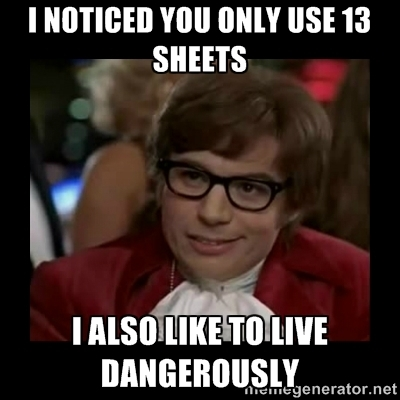
\includegraphics[width=\linewidth]{dangerously.jpg}
\end{center}
\end{multicols}
\end{document}
